% Options for packages loaded elsewhere
% Options for packages loaded elsewhere
\PassOptionsToPackage{unicode}{hyperref}
\PassOptionsToPackage{hyphens}{url}
\PassOptionsToPackage{dvipsnames,svgnames,x11names}{xcolor}
%
\documentclass[
  british,
  a4paper,
]{article}
\usepackage{xcolor}
\usepackage{amsmath,amssymb}
\setcounter{secnumdepth}{-\maxdimen} % remove section numbering
\usepackage{iftex}
\ifPDFTeX
  \usepackage[T1]{fontenc}
  \usepackage[utf8]{inputenc}
  \usepackage{textcomp} % provide euro and other symbols
\else % if luatex or xetex
  \usepackage{unicode-math} % this also loads fontspec
  \defaultfontfeatures{Scale=MatchLowercase}
  \defaultfontfeatures[\rmfamily]{Ligatures=TeX,Scale=1}
\fi
\usepackage{lmodern}
\ifPDFTeX\else
  % xetex/luatex font selection
\fi
% Use upquote if available, for straight quotes in verbatim environments
\IfFileExists{upquote.sty}{\usepackage{upquote}}{}
\IfFileExists{microtype.sty}{% use microtype if available
  \usepackage[]{microtype}
  \UseMicrotypeSet[protrusion]{basicmath} % disable protrusion for tt fonts
}{}
\makeatletter
\@ifundefined{KOMAClassName}{% if non-KOMA class
  \IfFileExists{parskip.sty}{%
    \usepackage{parskip}
  }{% else
    \setlength{\parindent}{0pt}
    \setlength{\parskip}{6pt plus 2pt minus 1pt}}
}{% if KOMA class
  \KOMAoptions{parskip=half}}
\makeatother
% Make \paragraph and \subparagraph free-standing
\makeatletter
\ifx\paragraph\undefined\else
  \let\oldparagraph\paragraph
  \renewcommand{\paragraph}{
    \@ifstar
      \xxxParagraphStar
      \xxxParagraphNoStar
  }
  \newcommand{\xxxParagraphStar}[1]{\oldparagraph*{#1}\mbox{}}
  \newcommand{\xxxParagraphNoStar}[1]{\oldparagraph{#1}\mbox{}}
\fi
\ifx\subparagraph\undefined\else
  \let\oldsubparagraph\subparagraph
  \renewcommand{\subparagraph}{
    \@ifstar
      \xxxSubParagraphStar
      \xxxSubParagraphNoStar
  }
  \newcommand{\xxxSubParagraphStar}[1]{\oldsubparagraph*{#1}\mbox{}}
  \newcommand{\xxxSubParagraphNoStar}[1]{\oldsubparagraph{#1}\mbox{}}
\fi
\makeatother


\usepackage{longtable,booktabs,array}
\newcounter{none} % for unnumbered tables
\usepackage{calc} % for calculating minipage widths
% Correct order of tables after \paragraph or \subparagraph
\usepackage{etoolbox}
\makeatletter
\patchcmd\longtable{\par}{\if@noskipsec\mbox{}\fi\par}{}{}
\makeatother
% Allow footnotes in longtable head/foot
\IfFileExists{footnotehyper.sty}{\usepackage{footnotehyper}}{\usepackage{footnote}}
\makesavenoteenv{longtable}
\usepackage{graphicx}
\makeatletter
\newsavebox\pandoc@box
\newcommand*\pandocbounded[1]{% scales image to fit in text height/width
  \sbox\pandoc@box{#1}%
  \Gscale@div\@tempa{\textheight}{\dimexpr\ht\pandoc@box+\dp\pandoc@box\relax}%
  \Gscale@div\@tempb{\linewidth}{\wd\pandoc@box}%
  \ifdim\@tempb\p@<\@tempa\p@\let\@tempa\@tempb\fi% select the smaller of both
  \ifdim\@tempa\p@<\p@\scalebox{\@tempa}{\usebox\pandoc@box}%
  \else\usebox{\pandoc@box}%
  \fi%
}
% Set default figure placement to htbp
\def\fps@figure{htbp}
\makeatother



\ifLuaTeX
\usepackage[bidi=basic,shorthands=off]{babel}
\else
\usepackage[bidi=default,shorthands=off]{babel}
\fi
\ifLuaTeX
  \usepackage{selnolig} % disable illegal ligatures
\fi


\setlength{\emergencystretch}{3em} % prevent overfull lines

\providecommand{\tightlist}{%
  \setlength{\itemsep}{0pt}\setlength{\parskip}{0pt}}



 


\makeatletter
\@ifpackageloaded{tcolorbox}{}{\usepackage[skins,breakable]{tcolorbox}}
\@ifpackageloaded{fontawesome5}{}{\usepackage{fontawesome5}}
\definecolor{quarto-callout-color}{HTML}{909090}
\definecolor{quarto-callout-note-color}{HTML}{0758E5}
\definecolor{quarto-callout-important-color}{HTML}{CC1914}
\definecolor{quarto-callout-warning-color}{HTML}{EB9113}
\definecolor{quarto-callout-tip-color}{HTML}{00A047}
\definecolor{quarto-callout-caution-color}{HTML}{FC5300}
\definecolor{quarto-callout-color-frame}{HTML}{acacac}
\definecolor{quarto-callout-note-color-frame}{HTML}{4582ec}
\definecolor{quarto-callout-important-color-frame}{HTML}{d9534f}
\definecolor{quarto-callout-warning-color-frame}{HTML}{f0ad4e}
\definecolor{quarto-callout-tip-color-frame}{HTML}{02b875}
\definecolor{quarto-callout-caution-color-frame}{HTML}{fd7e14}
\makeatother
\makeatletter
\@ifpackageloaded{caption}{}{\usepackage{caption}}
\AtBeginDocument{%
\ifdefined\contentsname
  \renewcommand*\contentsname{Table of contents}
\else
  \newcommand\contentsname{Table of contents}
\fi
\ifdefined\listfigurename
  \renewcommand*\listfigurename{List of Figures}
\else
  \newcommand\listfigurename{List of Figures}
\fi
\ifdefined\listtablename
  \renewcommand*\listtablename{List of Tables}
\else
  \newcommand\listtablename{List of Tables}
\fi
\ifdefined\figurename
  \renewcommand*\figurename{Figure}
\else
  \newcommand\figurename{Figure}
\fi
\ifdefined\tablename
  \renewcommand*\tablename{Table}
\else
  \newcommand\tablename{Table}
\fi
}
\@ifpackageloaded{float}{}{\usepackage{float}}
\floatstyle{ruled}
\@ifundefined{c@chapter}{\newfloat{codelisting}{h}{lop}}{\newfloat{codelisting}{h}{lop}[chapter]}
\floatname{codelisting}{Listing}
\newcommand*\listoflistings{\listof{codelisting}{List of Listings}}
\makeatother
\makeatletter
\makeatother
\makeatletter
\@ifpackageloaded{caption}{}{\usepackage{caption}}
\@ifpackageloaded{subcaption}{}{\usepackage{subcaption}}
\makeatother
\usepackage{bookmark}
\IfFileExists{xurl.sty}{\usepackage{xurl}}{} % add URL line breaks if available
\urlstyle{same}
% fallback for those not using the hyperref driver hyperxmp:
\makeatletter
\@ifundefined{xmpquote}{\newcommand{\xmpquote}[1]{#1}}{}
\makeatother
\hypersetup{
  pdftitle={Currency divergence scenarios for central Europe},
  pdfauthor={Carlos Galindo},
  pdflang={en-GB},
  colorlinks=true,
  linkcolor={blue},
  filecolor={Maroon},
  citecolor={Blue},
  urlcolor={Blue},
  pdfcreator={LaTeX via pandoc}}


\title{Currency divergence scenarios for central Europe}
\usepackage{etoolbox}
\makeatletter
\providecommand{\subtitle}[1]{% add subtitle to \maketitle
  \apptocmd{\@title}{\par {\large #1 \par}}{}{}
}
\makeatother
\subtitle{A quarterly-projection model extended with
political-credibility and capital-flow risk terms, used to frame how
neighbouring currencies could part ways}
\author{Carlos Galindo}
\date{}
\begin{document}
\maketitle


\begin{tcolorbox}[enhanced jigsaw, arc=.35mm, bottomrule=.15mm, breakable, colback=white, colframe=quarto-callout-note-color-frame, left=2mm, leftrule=.75mm, opacityback=0, rightrule=.15mm, toprule=.15mm]

\vspace{-3mm}\textbf{At a glance}\vspace{3mm}

\begin{itemize}
\tightlist
\item
  \textbf{Question.} When two neighbouring currencies look alike on
  interest rates and growth, what makes one of them break away, and can
  that be put into a scenario with probabilities attached?
\item
  \textbf{Approach.} A standard small-open-economy projection model,
  extended with a political-credibility term, a veto-friction term and a
  short-run capital-flow term, then run as simulations for Poland and
  four other economies.
\item
  \textbf{Finding.} Interest differentials alone mis-state the picture.
  Adding the two risk terms makes the exchange-rate path depend on
  governance and on who holds the debt, and it turns a single forecast
  into a set of weighted scenarios.
\item
  \textbf{Why it matters.} Divergence in a region is usually a story
  about institutions and flows as much as about policy rates; a scenario
  tool has to carry both.
\end{itemize}

\end{tcolorbox}

\subsection{The question}\label{the-question}

Central European currencies are often treated as a bloc. They share an
export base, an exposure to the euro area and a similar sensitivity to
global risk appetite. Yet in 2025 and 2026 they did not move together,
and the standard explanation, a gap in policy rates, accounts for only
part of the difference.

The practical question was a scenario one. Given a set of neighbouring
economies, which political and financial conditions would make one
currency depreciate relative to another over the next twelve months, how
likely is each path, and what would an investor or a policy analyst want
to watch to know which path is under way? The obvious approach, a
uncovered-interest-parity forecast with a fixed risk premium, treats the
premium as a constant. That is the weakest assumption in the model,
because the premium is exactly what moves when governance changes or
when a leveraged holder of government bonds has to sell.

\subsection{Approach}\label{approach}

\textbf{The base model.} The starting point is the family of
macroeconomic models studied earlier in the career break: the
three-equation model of an IS curve, a Phillips curve and a policy rule,
extended to a quarterly projection model for a small open economy. In
that setting the exchange rate is pinned down by interest parity, with
the expected change in the currency equal to the interest differential
less a risk premium.

\textbf{Two extensions.} The risk premium is split into two parts that
behave differently.

\begin{itemize}
\tightlist
\item
  A \emph{structural} premium that depends on three political
  primitives: the credibility of the government's commitments, the
  friction caused by veto players and divided institutions, and
  exogenous shocks, chiefly to the fiscal position. Credibility is
  scored on a zero-to-one scale; a high score shrinks the premium, a low
  score widens it.
\item
  A \emph{tactical} premium for short-run capital-flow risk. It rises
  with global risk aversion, with the share of illiquid assets held by
  non-bank financial institutions that may be forced to sell in a
  stress, and with the same political friction measure.
\end{itemize}

The policy rule and the Phillips curve also take the premiums as inputs,
so a rise in either one feeds back into inflation and into the interest
rate the central bank chooses. A fiscal block links the sovereign spread
to debt, to fiscal shocks, to the shortfall in credibility and to the
tactical premium.

\textbf{From model to scenarios.} The model is run forward by simulation
rather than solved once. Drivers are drawn jointly, with heavy tails and
positive dependence between global risk appetite, fiscal shocks and
political friction, because those things tend to arrive together. In the
worked case, a logistic link turns the drivers into the probability that
the economy enters a tail regime, and in that regime sovereign yields
jump by a large, uncertain amount while outside it they move modestly.
Bond returns at several maturities follow from the yield shock and the
duration, which gives expected outcomes, percentiles and
tail-conditional losses rather than a point forecast.

\textbf{Inputs and checks.} The worked case, Poland against its regional
peers, used a snapshot of late-2025 public market and fiscal data. The
weights linking drivers to premiums are illustrative calibrations,
chosen so that the tactical premium lands in a plausible range of basis
points for typical inputs, and they are exposed as parameters rather
than fixed. Where an input was missing, a timely proxy was substituted
and the substitution recorded; official figures more than a month old
were flagged as outdated.

\subsection{What the work shows}\label{what-the-work-shows}

\textbf{A worked case.} The Polish inputs combined a general-government
deficit of 6.8 per cent of GDP, a high political-friction score
reflecting a clash between the president and the government, and a
ten-year yield of 5.184 per cent against 4.578 per cent for the Czech
benchmark. The yield gap over the Czech benchmark is the observable that
the model treats as a term premium to be explained. The inputs mattered
less than the structure: they showed which drivers carried the weight.
Fiscal shocks and tactical flow risk moved the tail probability; the
political term moved the tactical premium and the structural premium
together, so it counted twice, which is the intended behaviour but also
the reason to treat its calibration with care.

\textbf{A cross-rate exercise.} A smaller simulation took two neighbours
with different credibility scores and different policy rates and asked
what a year of daily shocks does to the cross rate. The expected move is
the interest gap plus the difference in structural premiums, and the
simulated shocks spread the outcome around it. The exercise ended in
three scenario-conditional views, each with a stated probability: a
hedge against a sharp fall in one currency (60 per cent), a structural
view favouring the better-governed currency over the other (75 per cent
over twelve months), and a view that the bond curve would steepen as
monetary easing met a large deficit (65 per cent). Those probabilities
express the exercise's judgement, not a tested forecast.

The figures below use simulated data built to share the structure of the
analysis, and show the three things a reader would want to see.

\begin{figure}

\centering{

\pandocbounded{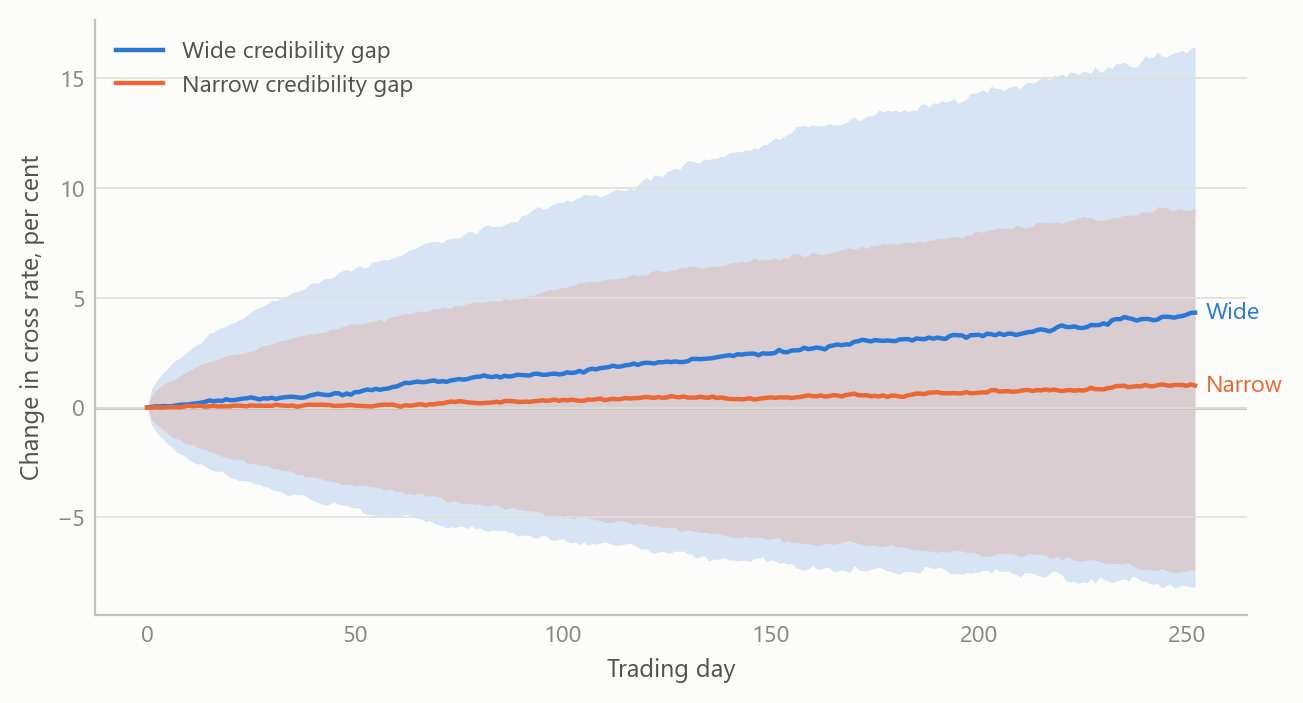
\includegraphics[keepaspectratio]{index_files/figure-latex/fig-cross-rate-output-1.png}}

}

\caption{\label{fig-cross-rate}Simulated twelve-month cross-rate paths
for two neighbours: a wide credibility gap versus a narrow one
(simulated data).}

\end{figure}%

The wide-gap case shifts the whole distribution and widens it, so the
spread of outcomes is wider as well as the central path being different.
That is the point of carrying a premium that responds to governance: the
risk is in the spread of outcomes, not only in the average.

\begin{figure}

\centering{

\pandocbounded{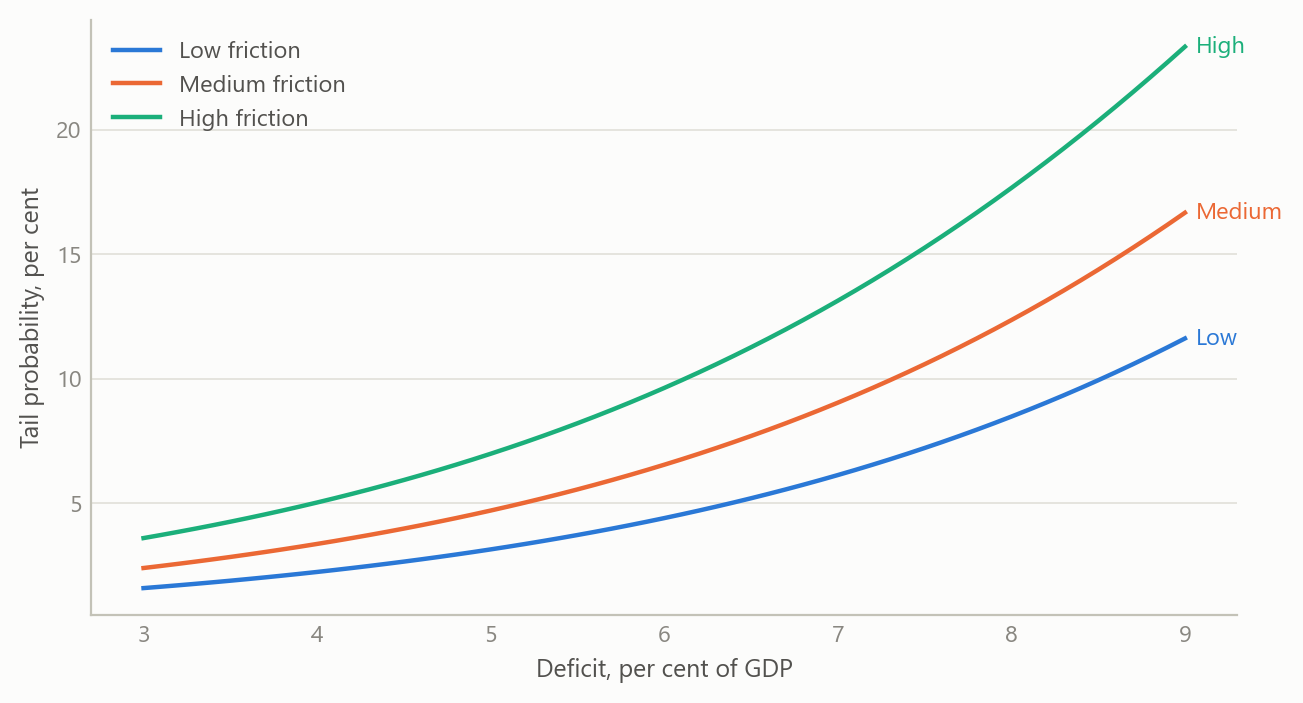
\includegraphics[keepaspectratio]{index_files/figure-latex/fig-tail-output-1.png}}

}

\caption{\label{fig-tail}Simulated probability of a tail regime as the
fiscal deficit widens, at three levels of political friction (simulated
data).}

\end{figure}%

The curves accelerate as the deficit widens, and political friction
lifts the whole curve. Because the link is non-linear, the same rise in
friction adds more probability where the deficit is already large.

\begin{figure}

\centering{

\pandocbounded{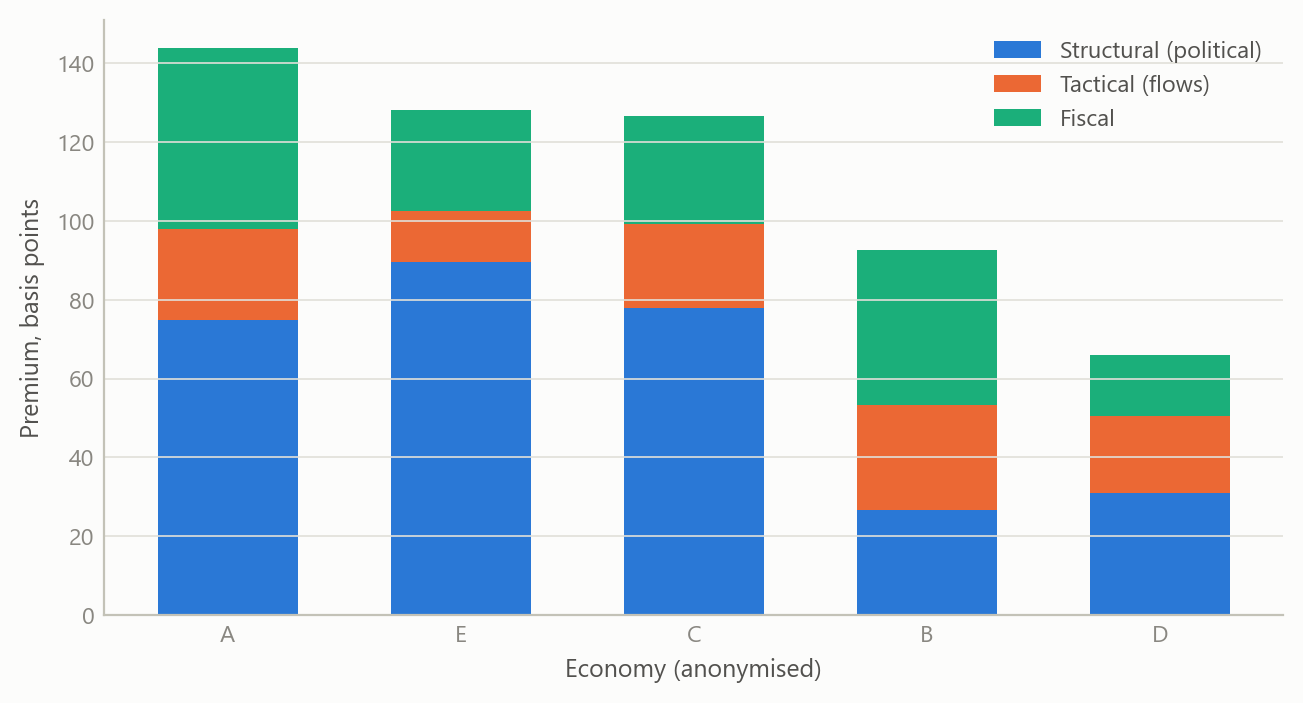
\includegraphics[keepaspectratio]{index_files/figure-latex/fig-premium-output-1.png}}

}

\caption{\label{fig-premium}Simulated decomposition of the sovereign
risk premium across five economies into structural, tactical and fiscal
parts (simulated data).}

\end{figure}%

Two economies with the same total premium can have very different parts,
and the parts imply different watch-lists: a mostly tactical premium can
reverse within weeks, a mostly structural one will not.

\subsection{Insights}\label{insights}

\begin{enumerate}
\def\labelenumi{\arabic{enumi}.}
\tightlist
\item
  \textbf{The risk premium is the model.} Holding it constant is a
  decision to ignore the political and financial channels. Splitting it
  into a slow structural part and a fast tactical part lets the same
  model explain a gradual drift and a sudden break.
\item
  \textbf{Political terms count twice, on purpose.} Friction raises both
  the structural and the tactical premium. That is realistic, since a
  standoff both worsens the long-run outlook and makes fast money leave,
  but it means results are sensitive to one parameter and should be
  shown with sensitivity ranges.
\item
  \textbf{Dependence matters more than any single driver.} Global risk
  appetite, fiscal shocks and political friction arrive together, so
  independent draws understate the tail. Heavy-tailed joint draws are
  the cheaper fix.
\item
  \textbf{Scenarios beat point forecasts for decisions.} A set of
  weighted paths, each with a named trigger, is something a user can
  monitor; a single number is not.
\item
  \textbf{Calibration should be visible.} Illustrative weights are
  acceptable if they are exposed and labelled. The earlier version of
  the worked case overwrote the computed tactical premium with a sourced
  figure; removing that override kept the results driven by the inputs
  rather than by the answer expected.
\end{enumerate}

\subsection{Scope and next steps}\label{scope-and-next-steps}

The framework is built to turn an argument about policy credibility and
political risk into explicit, comparable scenario probabilities for
currencies that share fundamentals but diverge, with each judgement
visible as a weight or a score.

The natural extensions are three. First, calibrated outputs for all five
economies. Second, driver weights estimated on a cross-section of
economies, and post-shock dynamics in the tail-regime simulation. Third,
an out-of-sample test of whether the credibility score improves
exchange-rate forecasts against a plain interest-parity benchmark.

The full framework can be discussed on request.

\subsection{About the evidence}\label{about-the-evidence}

The work was done between 2025 and 2026 on public macro, fiscal and
market data for Poland and four other economies. The worked case rests
on a late-2025 snapshot. The three figures are simulated, built to share
the structure of the analysis (a twelve-month horizon at daily
frequency, a logistic tail link, five economies); none shows a real
estimate.

Figures and tables marked \emph{simulated} are generated from simulated
data built to share the structure of the analysis (its variables,
horizons and frequencies). They show how each method works and what its
output looks like. Results stated in the text, and figures that give a
source, are the project's own. Methods are described at the level of a
methods section. Code and data pipelines are not reproduced here.




\end{document}
